\section{Cryptographie: méthodes}
Les problèmes de cryptographie reposent tous sur une branche des
mathématiques désignée sous le nom de \emph{théorie des
  nombres}\footnote{Il y a quelque chose de piquant là-dedans: avant
  l'apparition des méthodes de cryptographie modernes, les théoriciens
  des nombres disaient  à-peu-près \og Ça ne sert à rien, et donc les
  militaires ne vont pas se servir de mes recherches\fg.}. Parmi les
domaines d'études de la théorie des nombres figure tout ce qui touche
aux nombres premiers\footnote{Rappelons: un nombre entier est premier
  s'il n'est pas divisible par un nombre plus petit que lui. Par
  exemple: 2, 3, 5, 11, 13, 17 sont premiers, mais pas 4, 8, 15
  etc. La suite des nombres premiers est infinie et donc il en existe
  d'aussi grands qu'on veut.}.


\subsection{Crytographie symétrique}
Il faut s'assurer que quelqu'un qui ne connaît pas la clé ne pourra
pas la découvrir. Un des standards actuels est AES (voir \cite{aes}
(assez technique)).
\subsection{Cryptographie asymétrique}
Tous les algorithmes de cryptographie asymétrique sont basés sur le
même principe:
\begin{enumerate}
  \item Fabriquer la clé \emph{privée} est un problème facile, c'est à dire
    un problème qu'on peut résoudre en un temps calcul très limité.
  \item La clé \emph{publique} est fabriquée à partir de la clé privée, là
    aussi en résolvant un problème peu coûteux.
  \item \textbf{Mais le calcul inverse}, c'est à dire celui de
    retrouver la clé privée à 
    partir de la clé publique, 
    s'il est théoriquement possible, demande un temps calcul
    totalement inaccessible.
\end{enumerate}
Un autre propriété souhaitable est l'adaptabilité: même si les
ordinateurs et les algorithmes disponibles pour \emph{attaquer} la méthode
progressent, on doit pouvoir en rester maître en n'augmentant que peu la
complexité des calculs nécessaires pour pouvoir continuer à crypter et à
décrypter les messages sans risques.
\subsection{Complexité d'un algorithme}
La complexité d'un algorithme est le nombre d'opérations qu'il met en
{\oe}uvre, en fonction de la taille du problème à résoudre. Voici un
exemple assez simple:

\subsubsection{Complexité de la multiplication} On a tous appris à faire
des multiplications:

\begin{boxedminipage}{0.3\textwidth}
\begin{tabular}{ccccc}
        &&2&3&1\\
        &$\times$&1&2&4\\
        \hline
        &&9&2&4\\
        &4&6&2\\
        2&3&1\\
        \hline
        2&8&6&4&4\\
\end{tabular}
\end{boxedminipage}
\hspace*{0.02\textwidth}
\begin{minipage}{0.6\textwidth}
  Quelles sont les opérations? Il y a (exemple à gauche):
  \begin{itemize}
    \item des multiplications entre
      chiffres ($4 \times 1$, $4 \times 3$ etc.),
    \item des additions.
  \end{itemize}
      Ici
  on fait $3 \times 3$ multiplications entre
  chiffres. Les additions 
  sont  au maximum de $8$, car il peut y avoir des retenues.
\end{minipage}


Mais ce qu'on veut, c'est savoir comment cela se comporte quand on
multiplie des nombres de $n$ chiffres ($n=4,\ 5,\ 6,\, \cdots,
\ 100000, \cdots$) entre eux. On veut une estimation valable pour tout $n$.

Il est assez facile de compter les multiplications entre chiffres: il
y en a exactement $n^2$ (ça se vérifie facilement sur l'exemple
ci-dessus pour $n=3$).
Pour les additions, c'est un peu plus délicat, mais il y en a au
maximum $n^2 -1$ (ça dépend du nombre de retenues), soit au total
(additions et multiplications) de l'ordre de  $2 \times n^2$
opérations\footnote{ 
Remarquez que le
produit de deux nombres d'un million de chiffres demande environ 2000
milliards d'opérations ($2^{12}$); avec une machine qui tourne à 3 Ghz, cela va
demander environ $2 \times 10^{12}/(3\times 10^9)\simeq 666$ secondes.
\emph{Mais on peut faire une partie importante du calcul en parallèle
  (comment?) et gagner un facteur proche de 4 avec 4 c{\oe}urs, par exemple.}
}.

\paragraph{Implication  pratique:} ce coût implique simplement que,
\emph{quand on double le nombre de chiffres, le nombre d'opérations est
multiplié par $4$}. En général on dira que la complexité d'un
algorithme est, par exemple, en $n^2$, négligeant le facteur
muliplicatif ($2$ dans ce qu'on a vu), car ce qui compte, c'est bien
comment la difficulté croit quand $n$ augmente. 

\smallskip

\noindent\fbox{%
    \parbox{\textwidth}{
\begin{center}
  \emph{\bfseries Le coût de la multiplication de deux nombres de
    $\pmb{n}$ chiffres est 
  de l'ordre de $\pmb{n^2}$.}
\end{center}
}}\medskip



\subsubsection{Comparer des algorithmes} Il doit être clair que, si
pour résoudre le même problème on a deux algorithmes de complexités
différentes (par exemple $n^3$ et $n^2$), le plus rapide ($n^2$) est
le plus intéressant.


\subsubsection{Les problèmes trop coûteux} Évidemment, si les seuls
algorithmes dont on dispose pour résoudre un problème ont un  coût qui
croit très vite quand la taille du problème augmente, le 
problème devient difficile, voire même impossible  à résoudre.

Parmi ces problèmes les \emph{pires} sont ceux qui ont un coût dit
\emph{non polynomial}. Pour ces algorithmes, et pour une valeur $p$
\emph{quelconque}, si $n$ est assez grand, alors le coût devient
supérieur à $n^p$. De façon plus explicite, si $n$ est assez grand, le
coût deviendra supérieur disons à $n^{50000}$ ou pour une autre valeur
de $n$, il deviendra aussi supérieur à $n^{100 000}$ etc.


Parmi les possibilités, une est que le coût soit
exponentiel
(mais ce n'est pas la seule possibilité). L'exponentielle de $n$
est\footnote{Pour en finir avec l'exponentielle à toutes les sauces,
  voir \cite{sarko}.}:

$$\exp(n)= 1+ n + \frac{n^2}{2}+ \frac{n^3}{2 \times 3}+ \frac{n^4}{2
  \times 3 \times 4}+
\cdots+ \frac{n^p}{p!}+ \frac{n^{p+1}}{(p+1)!}+\ldots ,$$

avec $p! = 1\times 2\times 3\times \ldots \times (p-1)  \times p$.

Si vous comparez $\exp(n)$ à $n^p$ vous voyez que $
\frac{n^{p+1}}{(p+1)!}$ divisé par $n^p$ qui est égal à
$\frac{n}{(p+1)!}$, devient aussi grand qu'on
veut (c'est proportionnel à $n$). On dit alors que l'exponentielle
croit plus vite que tout polynôme.

\emph{Les problèmes qui ont un coût non polynomial ne peuvent pas être
  résolus, dès que la taille $n$ du problème devient grande.}

Ce qui est une catastrophe dans la vie courante est à la base des
méthodes modernes  de cryptographie.

\subsection{Une idée de cryptographie asymétrique} C'est l'idée qui
est derrière le système RSA (Ronald Rivest, Adi Shamir et Leonard
Adleman, 1983), mais la réalisation est plus complexe que ce qui est
expliqué ci-dessous (pour une explication détaillée --technique--,
voir \cite{rsa})\footnote{RSA est considéré comme dépassé, mais reste
  un très bon exemple.}.

\begin{enumerate}
  \item On choisit deux \emph{grands nombres premiers} $a$ et $b$ (par exemple,
    chacun ayant plus de 120 chiffres). Curieusement, c'est facile: on a un
    algorithme rapide pour cela. Ces deux nombres définissent la
    \textbf{clé privée}. 
  \item On les multiplie entre eux. En utilisant l'algorithme de
    multiplication classique, pour des nombres de $120$ chiffres, cela
    coûte environ $2 \times 120 \times 120 = 28800$ 
    opérations, autant dire rien ou presque\footnote{Et si on veut
      multiplier entre eux des nombres vraiment très grands, il existe
      des algorithmes beaucoup plus rapides: le plus simple est
      l'algorithme de Karatsuba (voir \cite{Karatsuba}); les plus
      performants utilisent la plus grande invention algorithmique du
      XX\ieme siècle, la Transformée de Fourier
      Rapide.}. \textbf{C'est ce nombre 
      qui va définir la clé publique}.
\end{enumerate}
    
Car la factorisation de $p = a \times b$, c'est à dire \emph{retrouver}
$a$ et $b$ connaissant leur produit $p$ est un problème difficile, à coût
non polynomial. 

\begin{minipage}{0.5\textwidth}
  \begin{center}
    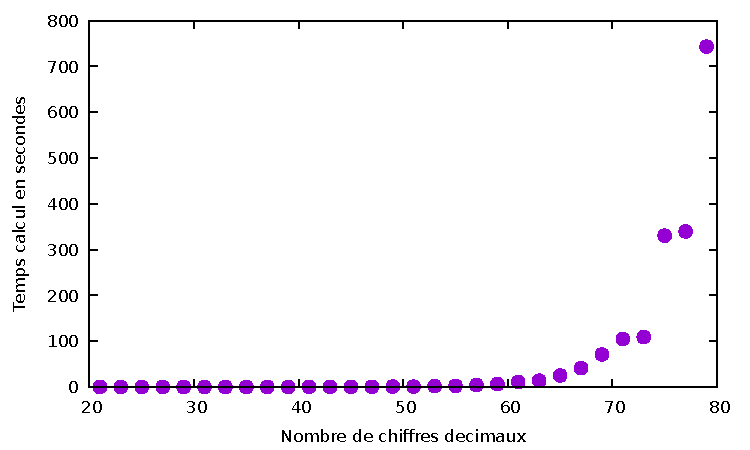
\includegraphics[width=0.8\textwidth]{images/facto.pdf}

    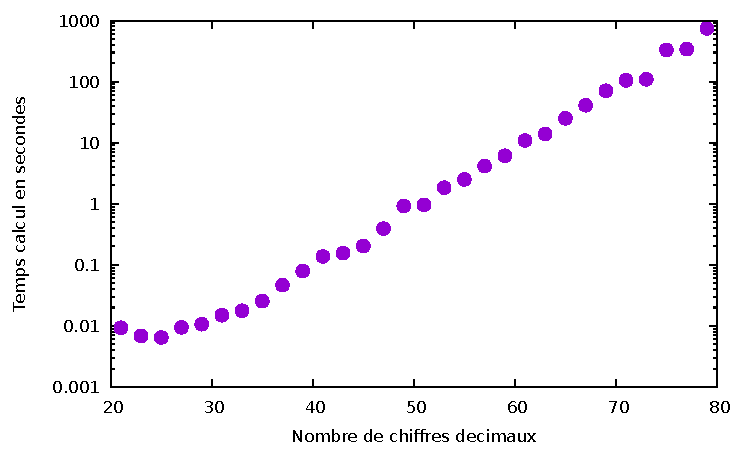
\includegraphics[width=0.8\textwidth]{images/factolog.pdf}
  \end{center}
\end{minipage}
\begin{minipage}{0.5\textwidth}
  Les graphiques ci-contre montrent le temps calcul (sur Intel
    I5, 3,4 Ghz)
  d'une factorisation 
  d'un nombre de $n$ chiffres ($n\leq 80$), produit de deux nombres
  premiers de $n/2$ chiffres. Le second graphique utilise une échelle
  logarithmique en 
  ordonnées pour présenter les mêmes résultats. Le calcul a été
    effectué avec le logiciel \ttt{SageMath} \cite{sagemath}  qui utilise la
    bibliothèque \ttt{Pari} (Bordeaux, \cite{Pari}).
\end{minipage}

\subsubsection{Quelques remarques}
\begin{itemize}
  \item Il n'existe aucune preuve du fait que la factorisation de deux
    nombres est un problème à coût non polynomial. Mais aucun
    algorithme n'a jamais été trouvé qui l'infirme et ce n'est pas
    faute d'avoir  cherché.
  \item Il existe une compétition de factorisation (voir \cite{rsafac}),
    une liste de nombres produits de deux nombres premiers, de taille
    croissante à factoriser. Le record actuel est le nombre RSA-250
    (250 chiffres décimaux), factorisé le 28 février 2020 par une
    équipe de l'INRIA à Nancy. Si vous arrivez a factoriser RSA-1024
    (1024 chiffres décimaux),
    vous gagnerez 100~000 \$.
  \item Les ordinateurs quantiques, s'ils existent un jour, pourront
    factoriser des nombres de $n$ chiffres avec un coût de
    l'ordre de $n^3$, ce qui invalidera les méthodes de
    cryptographie basées sur ce genre de principe\footnote{Pour
      l'instant les \og ordinateurs 
      quantiques\fg{} ont réussi à
      factoriser... $15$ (ils ont bien 
      trouvé que $15 = 5 \times 3$). Il reste donc un peu de temps
      avant de changer de méthode}.
  \item Le principe est une chose, sa réalisation pratique en est une
    autre. On n'a aucune preuve que \ttt{openssh} n'a pas de trou de
    sécurité ni de bug. Un a été découvert il y a quelque temps: le générateur
    aléatoire qui choisit les nombres premiers \emph{a} et \emph{b}
    était mal utilisé et il les sélectionnait dans un petit ensemble de
    nombres ce qui, théoriquement, aurait pu permettre de casser le
    chiffre RSA (avec une très, très grosse puissance de calcul).
\end{itemize}
    

